\documentclass{article}
\usepackage{tikz}
\usepackage{amsmath}
\usepackage{svg}
\usepackage{xcolor}
\usepackage[cache=false]{minted}
\usepackage{pdflscape}


\usetikzlibrary {arrows.meta,bending,positioning} 

\usetikzlibrary{shapes.geometric, shapes.arrows}
\usetikzlibrary{patterns}
\usetikzlibrary{quantikz2}
     \tikzset{operator/.append style={fill=white!0}}


\newsavebox{\incode} 
\newsavebox{\fmovecode}
\newsavebox{\fmoveqiskit}
\newsavebox{\nmovecode}
\newsavebox{\nmoveqiskit}
\newsavebox{\ffcapturecode}
\newsavebox{\ffcaptureqiskit}



\begin{document}

% Save tabular in a box
\savebox{\fmovecode}{%
    \begin{tabular}{l}
        board[i] = \textcolor{blue}{None} \\ 
        board[i+d1, i+d2] = \{\\
            \quad \textcolor{orange}{'color'} : \textcolor{blue}{red}, \\
            \quad \textcolor{orange}{'probability'} : \textcolor{blue}{0.5}, \\
            \quad \textcolor{orange}{'pawn'} : \textcolor{blue}{1}\} \\
    \end{tabular}
}

\savebox{\incode}{%
\begin{tabular}{l} 
    board[i] = \{\\ 
        \quad \textcolor{orange}{'color'} : \textcolor{blue}{red}, \\ 
        \quad \textcolor{orange}{'probability'} : \textcolor{blue}{1}, \\ 
        \quad \textcolor{orange}{'pawn'} : \textcolor{blue}{1} 
        \} 
    \end{tabular}
}

\savebox{\fmoveqiskit}{%
    \begin{tabular}{l} 
        circuit.cx(q[i], q[i+d1]) \\
        circuit.cx(q[i], q[i+d1]) \\
        circuit.h(q[i+d1]) \\
        circuit.h(q[i+d2]) \\
        circuit.x(q[i])
    \end{tabular}
}

\savebox{\nmovecode}{%
    \begin{tabular}{l}
        board[i] = \textcolor{blue}{None} \\ 
        board[i+d1, i+d2] = \{\\
            \quad \textcolor{orange}{'color'} : \textcolor{blue}{red}, \\
            \quad \textcolor{orange}{'probability'} : $\mathcolor{blue}{(1/2)^n}$, \\
            \quad \textcolor{orange}{'pawn'} : \textcolor{blue}{1}\} \\
    \end{tabular}
}

\savebox{\nmoveqiskit}{%
\begin{tabular}{l} 
    circuit.h(q[i]) \\
    circuit.cx(q[i], q[i+d1]) \\
    circuit.cx(q[i], q[i+d1]) \\
    circuit.h(q[i+d1]) \\
    circuit.h(q[i+d2]) \\
    circuit.x(q[i])
\end{tabular}
}

\savebox{\ffcapturecode}{%
    \begin{tabular}{l}
        board[i] = \textcolor{blue}{None} \\ 
        board[i+d1, i+d2+1] = \{\\
            \quad \textcolor{orange}{'color'} : \textcolor{blue}{red}, \\
            \quad \textcolor{orange}{'probability'} : $\mathcolor{blue}{(1/2)^n}$, \\
            \quad \textcolor{orange}{'pawn'} : \textcolor{blue}{1}\} \\
    \end{tabular}
}

\savebox{\ffcaptureqiskit}{%
\begin{tabular}{l} 
    circuit.h(q[i]) \\
    circuit.cx(q[i], q[i+d1]) \\
    circuit.cx(q[i], q[i+d1]) \\
    circuit.h(q[i+d1]) \\
    circuit.h(q[i+d2]) \\
    circuit.x(q[i])
\end{tabular}
}

    \begin{landscape}
        \begin{center}
            \begin{tabular}{||c c c c c||} 
            \hline
            Move name & Move & Python list & Quantum array & Qiskit \\ [0.5ex] 
            \hline\hline
            Initialize & 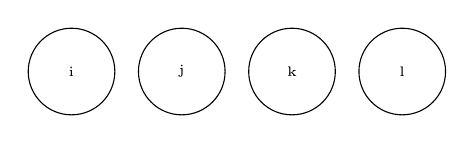
\begin{tikzpicture}
    \def\d{1.4}
    \def\size{1.1}
    \node(c1) [circle, draw, minimum size = \size cm] at (\d * 0,0) {\tiny i};
    \node(c2) [circle, draw, minimum size = \size cm] at (\d * 1,0) {\tiny j};
    \node(c3) [circle, draw, minimum size = \size cm] at (\d * 2,0) {\tiny k};
    \node(c4) [circle, draw, minimum size = \size cm] at (\d * 3,0) {\tiny l};
\end{tikzpicture} & $\text{board=[\textcolor{blue}{None}] * 32}$ & \begin{quantikz}[color=gray, scale=1.5]
    &\setwiretype{n} \lstick{\small$i\;$} &  \lstick{$\ket{0}$} & \setwiretype{q}& \\
    &\setwiretype{n} \lstick{\small$j\;$} &  \lstick{$\ket{0}$} &\setwiretype{q} &\\
    &\setwiretype{n} \lstick{\small$k\;$} &  \lstick{$\ket{0}$} &\setwiretype{q} &\\
    &\setwiretype{n} \lstick{\small$l\;$} &  \lstick{$\ket{0}$} &\setwiretype{q} &\\[-1em]
\end{quantikz} &  \begin{tabular}{l} q = QuantumRegister(10, \textcolor{orange}{'q'}) \\ circuit = QuantumCircuit(q)\end{tabular} \\ [1ex]
            \hline
            New pawn & \newsavebox{\newpawncircuit}
\newsavebox{\newpawnvis}
\newsavebox{\dice}

\savebox{\newpawncircuit}{
    \begin{quantikz}
        \lstick{$\ket{0}_0$} & \gate{X} & \rstick{$\ket{1}_0$}\\[-0.8em]
        \lstick{$\ket{0}_1$}& & \rstick{$\ket{0}_1$}\\
        \lstick{$\ket{0}_2$} &&\rstick{$\ket{0}_2$}\\
    \end{quantikz}
}

\savebox{\dice}{
    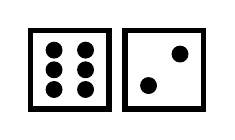
\begin{tikzpicture}
        \def\dielength{1}
        \def\dlwith{2}
        \def\dotsize{\dielength cm * 0.2}
        \node(die1) [rectangle, draw, line width = \dlwith pt, minimum width = \dielength cm, minimum height = \dielength cm] at (-\dielength/2-0.1*\dielength,0) {};
        
        \node [circle, draw, fill, minimum size = \dotsize, inner sep=0pt] at ($(die1) + (0.2 * \dielength,0.25*\dielength)$) {};
        \node [circle, draw, fill, minimum size = \dotsize, inner sep=0pt] at ($(die1) + (0.2 * \dielength,0*\dielength)$) {};
        \node [circle, draw, fill, minimum size = \dotsize, inner sep=0pt] at ($(die1) + (0.2 * \dielength,-0.25*\dielength)$) {};
        \node [circle, draw, fill, minimum size = \dotsize, inner sep=0pt] at ($(die1) + (-0.2 * \dielength,0.25*\dielength)$) {};
        \node [circle, draw, fill, minimum size = \dotsize, inner sep=0pt] at ($(die1) + (-0.2 * \dielength,0*\dielength)$) {};
        \node [circle, draw, fill, minimum size = \dotsize, inner sep=0pt] at ($(die1) + (-0.2 * \dielength,-0.25*\dielength)$) {};

        \node(die2) [rectangle, draw, line width = \dlwith pt, minimum width = \dielength cm, minimum height = \dielength cm] at (+\dielength/2+0.1*\dielength,0) {};
        \node [circle, draw, fill, minimum size = \dotsize, inner sep=0pt] at ($(die2) + (0.2 * \dielength,0.2*\dielength)$) {};
        \node [circle, draw, fill, minimum size = \dotsize, inner sep=0pt] at ($(die2) + (-0.2 * \dielength,-0.2*\dielength)$) {};
    \end{tikzpicture}
}

\savebox{\newpawnvis}{
    \begin{tikzpicture}
        \def\d{1.1}
        \def\size{0.8 cm}
        \node (arrow) [single arrow, draw, minimum width = 40 pt, single arrow head extend=3pt, minimum height=60 pt] at (0,0) {};
        \node (dice) [] at (0,0) {\scalebox{0.5}{\usebox{\dice}}};
        \node (c0l) [circle, draw, minimum size = \size] at ($(arrow.west) + (-2.5*\d,0)$) {0};
        \node (c1l) [circle, draw, minimum size = \size] at ($(arrow.west) + (-1.5*\d,0)$) {1};
        \node (c2l) [circle, draw, minimum size = \size] at ($(arrow.west) + (-0.5*\d,0)$) {2};
        
        \node (c0r) [circle, draw, minimum size = \size, pattern = horizontal lines, fill] at ($(arrow.east) + (0.5*\d,0)$) {};
        \node[circle, fill=white, inner sep=0.3mm, text=black] at ($(arrow.east) + (0.5*\d,0)$) {0};
        \node (c1r) [circle, draw, minimum size = \size] at ($(arrow.east) + (1.5*\d,0)$) {1};
        \node (c2r) [circle, draw, minimum size = \size] at ($(arrow.east) + (2.5*\d,0)$) {2};
    \end{tikzpicture}
}

\begin{tikzpicture}
    \node (circuit) [] at (0,0) {\scalebox{1.5}{\usebox{\newpawncircuit}}};
    \node (vis) [above] at ($(0,0.1)+(circuit.north)$) {\usebox{\newpawnvis}};
\end{tikzpicture} & \usebox{\incode} & \begin{quantikz}[color=gray, scale=1.5]
    &\setwiretype{n} \lstick{\small$i\;$} & \setwiretype{q}& \gate{X} & \\
    &\setwiretype{n} \lstick{\small$j\;$} &\setwiretype{q} & &\\
    &\setwiretype{n} \lstick{\small$k\;$} &\setwiretype{q} &&\\
    &\setwiretype{n} \lstick{\small$l\;$} &\setwiretype{q} &&\\[-1em]
\end{quantikz} & circuit.x[q[i]] \\
            \hline
            First move & \input{moves/first_move.tex} & \usebox{\fmovecode} & \begin{quantikz}[scale=1]
    \lstick{$\ket{1}_i$}        & \ctrl{1} & \swap{2} &  &\rstick{$\ket{0}$}\\
    \lstick{$\ket{0}_{i+d_1}$}  & \gate{H} &          & \ctrl{1} &\rstick[wires=2]{$\ket{01}+\ket{10}$}\\
    \lstick{$\ket{0}_{i+d_2}$}  &          & \swap{-2} & \targ{ }&
\end{quantikz} & \usebox{\fmoveqiskit} \\
            \hline
            nth move & \input{moves/pth_move.tex} & \usebox{\nmovecode} & \begin{quantikz}[color=gray, scale=1]
    \lstick{\small$i\;$}  &\gate{H} & \ctrl{1} & \ctrl{2} & \gate{X}& \\
    \lstick{\small$i+d1\;$} &    & \targ{ } &          & \gate{H}& \\
    \lstick{\small$i+d2\;$} &     &       & \targ{ } & \gate{H}& 
\end{quantikz} & \usebox{\nmoveqiskit} \\
            \hline
            \end{tabular}
        \end{center}
        \begin{center}
            \begin{tabular}{||c c c c c||} 
            \hline
            Move name & Move & Python list & Quantum array & Qiskit \\ [0.5ex] 
            \hline\hline
            full-full capture & 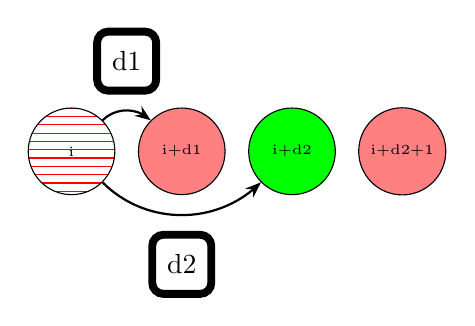
\begin{tikzpicture}
    \def\d{1.4}
    \def\size{1.1}
    \node(c1) [circle, draw, minimum size = \size cm, pattern={horizontal lines},pattern color=red] at (\d * 0,0) {\tiny i};
    \node(c2) [circle, draw, minimum size = \size cm, fill = red!50] at (\d * 1,0) {\tiny i+d1};
    \node(c3) [circle, draw, minimum size = \size cm, fill = green] at (\d * 2,0) {\tiny i+d2};
    \node(c4) [circle, draw, minimum size = \size cm, fill =red!50] at (\d * 3,0) {\tiny i+d2+1};

    \draw[draw, thick, -{Stealth[length=2mm]}]
    (c1) edge [bend left=45] node[pos=0.5, above, rectangle, draw, minimum width = 0.75 cm, minimum height = 0.75 cm, rounded corners, line width = 0.1 cm, yshift=0.2cm] {d1} (c2)
    (c1) edge [bend right=45] node[pos=0.5, below, rectangle, draw, minimum width = 0.75 cm, minimum height = 0.75 cm, rounded corners, line width = 0.1 cm, yshift=-0.2cm] {d2} (c3);
\end{tikzpicture} & \usebox{\ffcapturecode} & \begin{quantikz}[scale=1]
    \lstick{$\ket{1}_i$}        & \ctrl{1} & \swap{3}  &          &             &\rstick{$\ket{0}$}\\
    \lstick{$\ket{0}_{i+d_1}$}  & \gate{H} &           & \ctrl{2} &             &\rstick[wires=3]{$\ket{110}+\ket{001}$}\\
    \lstick{$\ket{1}_{i+d_2}$}  &          &           &          & \targ{ }    & \\
    \lstick{$\ket{0}_{i+d_2+1}$}&          & \swap{-3} & \targ{ } & \ctrl{-1}   &
\end{quantikz} & \usebox{\ffcaptureqiskit} \\
            \hline
            \end{tabular}
        \end{center}

    \end{landscape}
\end{document}
